\documentclass{standalone}
\usepackage{pgfplots}
\pgfplotsset{compat=newest}

\begin{document}
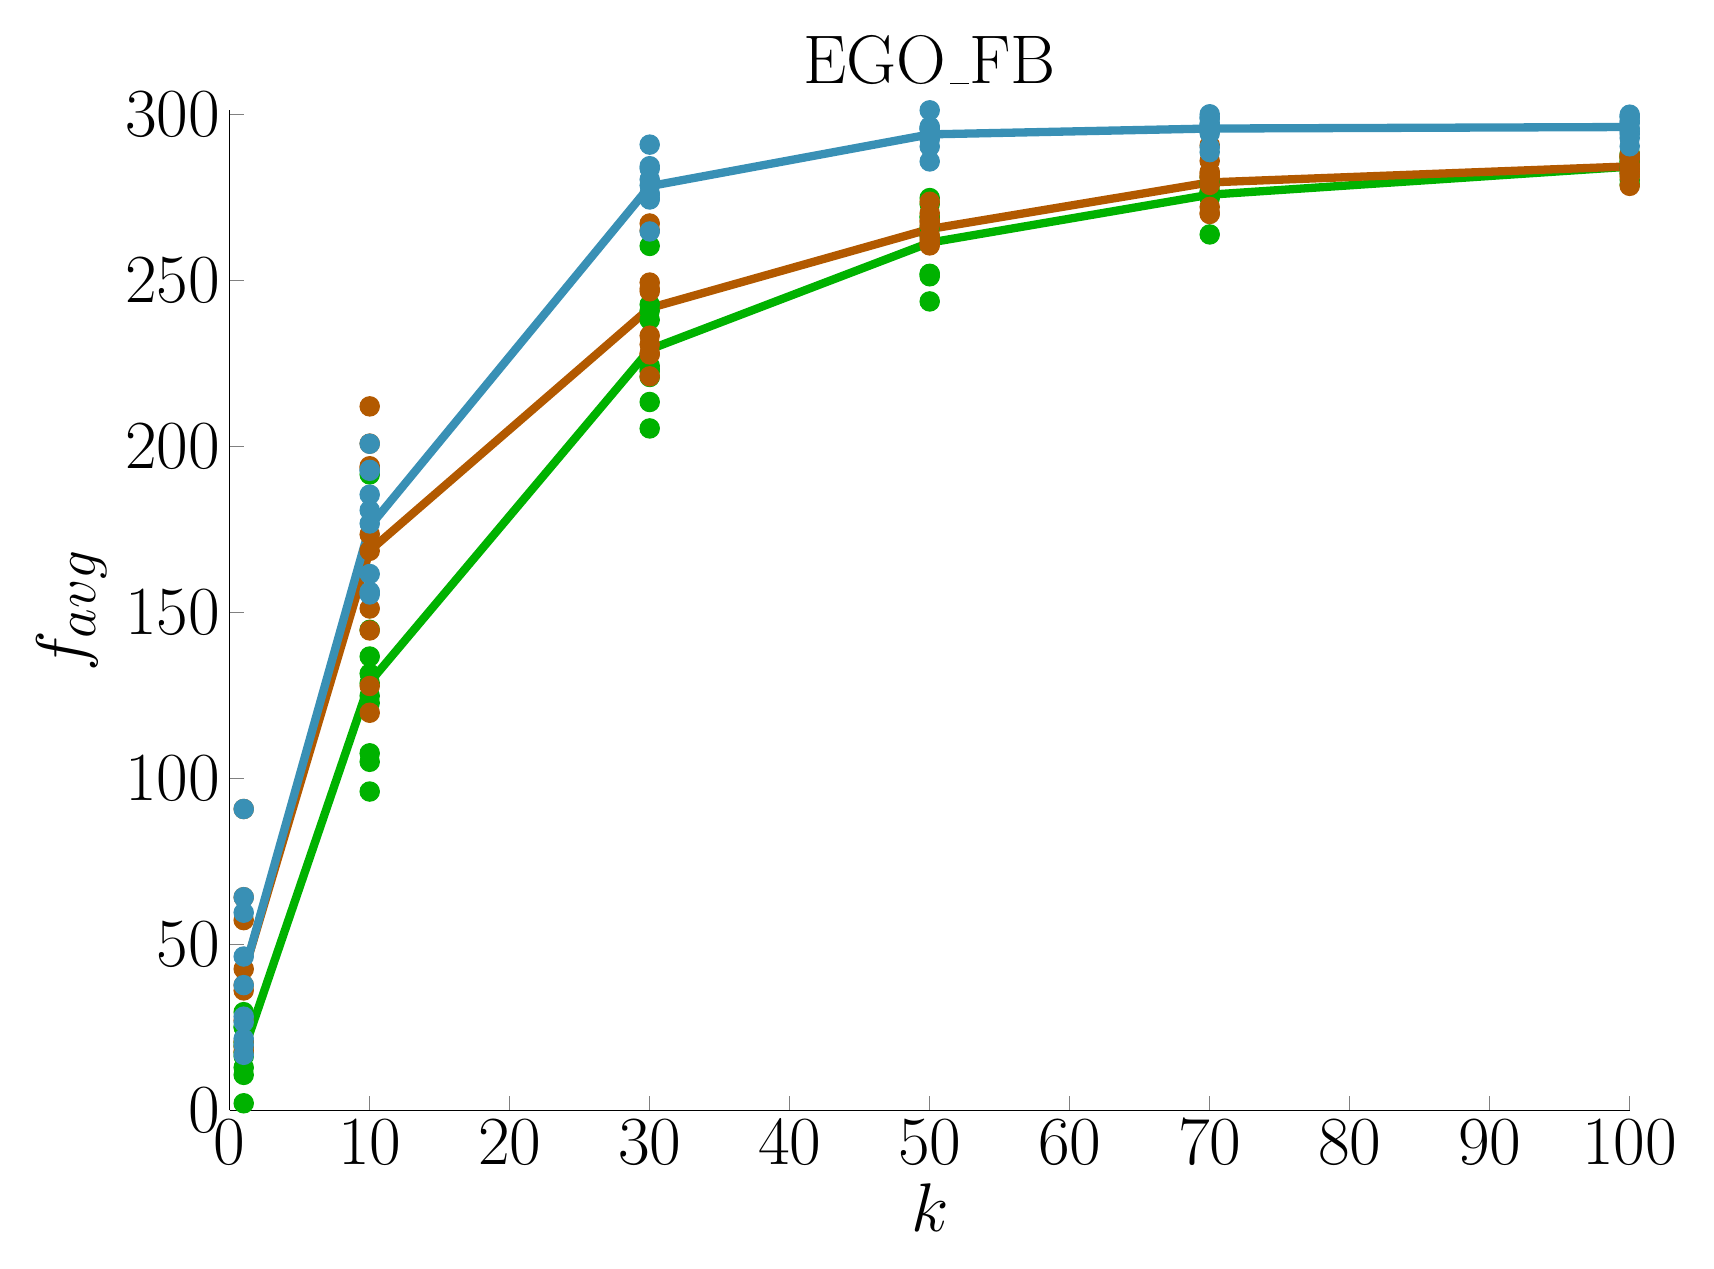
\begin{tikzpicture}

\begin{axis}[%
title style={font=\Huge},
title=EGO\_FB,
tick label style={font=\Huge},
label style={font=\Huge},
legend style={font=\Huge},
view={0}{90},
max space between ticks=50pt,
width=7in,
height=5in,
scale only axis,
xmin=0, xmax=100,
%xtick={0, 20, 40, 60, 80, 100},
xlabel={$k$},
ymin=0, ymax=301.28,
ylabel={$f_{avg}$},
major tick length=5pt,
axis lines*=left,
legend cell align=left,
clip=false]

\addplot [
only marks,
mark=*,
mark size=3.5pt,
color=green!70!black,
%solid,
%line width=2pt,
]
coordinates{
(1,2.12)(1,10.68)(1,12.88)(1,16.28)(1,17.44)(1,19.38)(1,20.46)(1,25.02)(1,25.16)(1,29.58)(10,96.04)(10,105.0)(10,107.56)(10,122.76)(10,124.86)(10,128.7)(10,131.56)(10,136.72)(10,144.76)(10,191.56)(30,205.44)(30,213.4)(30,220.94)(30,222.62)(30,223.36)(30,224.28)(30,238.16)(30,240.92)(30,242.78)(30,260.42)(50,243.7)(50,251.28)(50,251.86)(50,252.02)(50,263.22)(50,265.94)(50,268.94)(50,269.32)(50,273.02)(50,274.84)(70,263.88)(70,274.88)(70,275.32)(70,275.74)(70,276.18)(70,276.66)(70,276.74)(70,278.82)(70,279.24)(70,281.1)(100,278.96)(100,280.32)(100,282.24)(100,283.22)(100,284.06)(100,285.76)(100,285.94)(100,287.1)(100,287.22)(100,288.26)
};

\addplot [
only marks,
mark=*,
mark size=3.5pt,
color=orange!70!black,
%solid,
%line width=2pt,
]
coordinates{
(1,17.8)(1,19.14)(1,20.82)(1,27.1)(1,36.12)(1,37.72)(1,42.58)(1,57.3)(1,64.2)(1,90.78)(10,119.78)(10,127.84)(10,144.58)(10,151.18)(10,168.56)(10,173.5)(10,193.54)(10,194.04)(10,200.86)(10,212.08)(30,221.14)(30,227.74)(30,228.06)(30,230.7)(30,233.38)(30,246.76)(30,247.52)(30,249.38)(30,265.14)(30,267.18)(50,260.58)(50,261.04)(50,261.38)(50,262.34)(50,263.5)(50,266.64)(50,267.62)(50,268.02)(50,270.3)(50,273.72)(70,270.04)(70,270.36)(70,272.18)(70,278.8)(70,281.06)(70,281.52)(70,282.16)(70,282.68)(70,286.04)(70,290.78)(100,278.52)(100,281.32)(100,282.3)(100,283.16)(100,284.12)(100,284.88)(100,286.68)(100,287.32)(100,287.76)(100,287.8)
};

\addplot [
only marks,
mark=*,
mark size=3.5pt,
color=cyan!70!black,
%solid,
%line width=2pt,
]
coordinates{
(1,16.72)(1,19.74)(1,21.58)(1,26.56)(1,28.22)(1,37.72)(1,46.34)(1,59.54)(1,64.2)(1,90.78)(10,155.42)(10,156.02)(10,156.24)(10,161.58)(10,176.8)(10,180.8)(10,185.48)(10,192.66)(10,192.96)(10,200.82)(30,264.78)(30,274.42)(30,274.88)(30,275.74)(30,276.22)(30,278.68)(30,280.42)(30,283.74)(30,284.44)(30,290.94)(50,285.88)(50,290.38)(50,292.54)(50,292.9)(50,293.78)(50,295.56)(50,295.68)(50,295.92)(50,296.36)(50,301.28)(70,288.68)(70,290.14)(70,294.34)(70,295.52)(70,296.7)(70,296.98)(70,297.36)(70,298.82)(70,299.22)(70,300.08)(100,290.44)(100,292.96)(100,294.14)(100,294.92)(100,295.82)(100,297.52)(100,298.06)(100,299.3)(100,299.34)(100,299.96)
};
p
\addplot [
color=green!70!black,
solid,
line width=3pt
]
coordinates{
(1,17.9)(10,128.952)(30,229.232)(50,261.414)(70,275.856)(100,284.308)
};

\addplot [
color=orange!70!black,
solid,
line width=3pt
]
coordinates{
(1,41.356)(10,168.596)(30,241.7)(50,265.514)(70,279.562)(100,284.386)
};

\addplot [
color=cyan!70!black,
solid,
line width=3pt
]
coordinates{
(1,41.14)(10,175.878)(30,278.426)(50,294.028)(70,295.784)(100,296.246)
};


\end{axis}
\end{tikzpicture}
\end{document}
